% !TEX root = ./main.tex
\section{Work-Stealing}
\label{sec:wsmechanisms}

In this section, we introduce some formal notations and we present the WS algorithm that we study.

\subsection{Notation and definition}

We consider a discrete time model. 
The target parallel platform is composed of $p$ identical processors. We denote
by $\calW_{i}(t)\in\{0,1,\dots\}$
 the amount of work on processor $P_{i}$ at time $t$ (for
 $i\in\{1\dots p\}$).
 A unit of work corresponds to one unit of execution time.
 We denote the total amount of work on all processors by
 $\calW(t) = \sum_{i=1}^{p} \calW_{i}(t)$.
we assume that at $t=0$ the whole work is located on one processor, say $P_{1}$. 
The total amount of work at time $0$
is denoted by $\calW = \calW_{1}(0)$.

%
%
%\section{Task Models and Work-Stealing Algorithm}
%\label{sec:wsmechanisms}
%
%We consider a discrete time model of a parallel platform with $p$
%identical processors.  In this section, we introduce the two models of
%task dependence that we will study and how they affect the work
%stealing algorithm. 
%
%\subsection{Dependence between tasks}
%
%The tasks can be independent or constrained by a
%directed acyclic graph (DAG) of precedence. The total amount of
%processing work to complete all tasks is denoted by $\calW$. When the
%tasks have some dependencies, we denote by $D$ the critical path of
%the DAG (that corresponds to its depth).
%
%\subsubsection{Independent Tasks}
%
%Our first case of interest is to consider unitary independent
%tasks. For this case, we denote by $w_{i}(t)\in\N$ the number of units
%of work that processor $i$ has at time $t$ (for $i\in\{1\dots
%p\}$). At unit of work corresponds to one unit of execution time.  The
%total amount of work on all processors by
%$\calW(t) = \sum_{i=1}^{p} w_{i}(t)$.  At $t=0$ all work is on one
%processor. The total amount of work at time $0$ is
%$\calW = w_{1}(0)$.  In this model, all tasks are independent
%which means that when a processor steals from another processor, it
%could steal as many tasks as there are available. We will assume for
%this model that that each successful steal divides the work in two
%equal parts.
%
%\subsubsection{DAG of precedence}
%
%We consider a model similar to \cite{Arora2001,Denis2013} where the
%workload is composed of $\mathcal{W}$ unitary tasks that have precedence
%constraints represented by a DAG. This DAG has a single source that
%represents the first task and that is originally located on a given
%processor.  We consider that the scheduling is done as in
%\cite{Arora2001}: each processor maintains a double-ended queue
%(called deque) of activated tasks. If a processor has one or more task
%in its deque, it executes the tasks at the head of its deque. This
%takes one unit of time. After completion, a task might activates $0$,
%$1$ or $2$ tasks that are pushed at the end of the deque.  The
%activation tree is a binary tree whose shape depends on the execution
%of the algorithm. It is a subset of the original DAG and has the same
%critical path.  We define the height of node of this tree as
%follows. The height of the source as $D$ (\emph{i.e.}, the length of
%the critical path). The height of another task is equal to the length
%of its father minus one.  We assume when a processor steals work from
%another processor, it steals the activated tasks with the largest
%height.
%
%% ABP schedules the DAG $G$ as follows.  Each processor $i$
%% maintains a double-ended queue (called a deque) $Q_i$ of ready tasks.
%% At each slot, an active processor $i$ with a nonempty deque executes
%% the task at the bottom of its deque $Q_i$; once its execution is
%% completed, this task is popped from the bottom of the deque, enabling
%% --~\textit{i.e.} making ready~-- $0$, $1$ or $2$ child tasks that are
% pushed at the bottom of $Q_i$. At each top, an idle processor $j$ with
% an empty deque $Q_j$ becomes a thief: it performs a work request on
% another randomly chosen victim deque; if the victim deque contains
% ready tasks, then its top-most task is popped and pushed into the
% deque of one of its concurrent thieves.  If $j$ becomes active just
% after its work request, the work request is said to be
% successful. Otherwise, $Q_j$ remains empty and the work request fails
% which may occur in the three following situations: either the victim
% deque $Q_i$ is empty; or, $Q_i$ contains only one task currently in
% execution on $i$; or, due to contention, another thief performs a
% successful work request on $i$ simultaneously.


\subsection{Work stealing algorithm}

Work Stealing is a decentralized list scheduling algorithm where each
processor maintains its own local queue or deque of tasks to
execute. When a processor $i$ has nothing to execute, it selects
another processor $j$ uniformly at random and sends a work request to
it. When a processor $j$ receives this request, it answers by either
sending some of its work or by a fail response. 

\begin{figure}[tp!]
  %\hspace{-15pt}
  \centering
  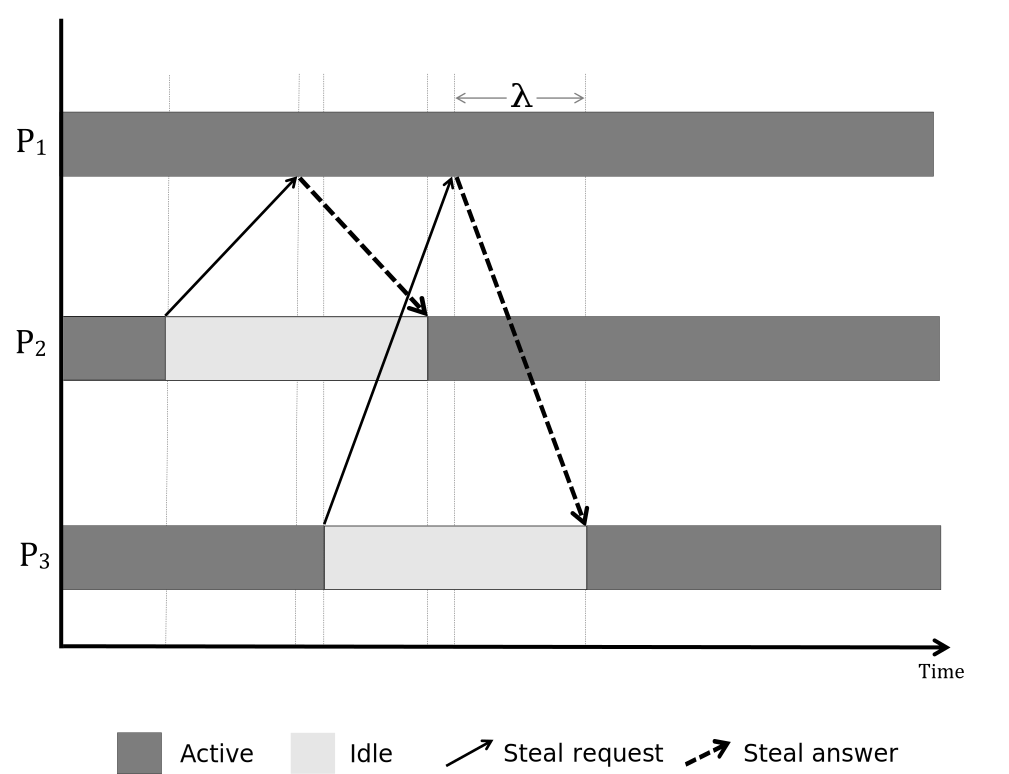
\includegraphics[width=0.6\linewidth]{figures/ws.pdf}
  \caption{Example of a work stealing execution with 3 processors} 
  \label{fig:workStealing}
\end{figure}




We analyze a model of WS algorithm that has the following features:
\begin{itemize}

\item \textbf{Latency:} All communication takes a time
  $\lambda\in\N^+$ that we call the latency.
  Figure~\ref{fig:workStealing} presents an example of Work Stealing
  execution with latency $\lambda$, A work request that is sent at
  time $t-\lambda$ by a thief will be received at time $t$ by the
  victim.  The thief will then receive an answer at time $t+\lambda$.
  As we consider a discrete-time model, we say that a work request
  arrives at time $t$ if it arrives between $t-1$ (not-included) and
  $t$.  This means that at time $t$, this work request is treated. We
  do not assume that the work requests are synchronized.  The number
  of incoming work requests at time $t$ is denoted by
  $R(t)\in\{0,1,\dots,p-1\}$. It is equal to the number of processors
  sending a work request at time $t - \lambda$.  When a processor $i$
  receives a work request from a thief $j$, it sends a part of its
  work to $j$. This communication takes again $\lambda$ units of time.
  The processor $j$ receives the work at time $t+\lambda$.  We denote
  by $s_{i}(t)$ the amount of work in transit from $P_i$ at time $t$.
  At end of the communication $s_{i}$ becomes 0 until another work
  request arrives.
  
\item \textbf{Single work transfer:} We assume that a processor can
  send some work to at most one processor at a time.  While the
  processor sends work to a thief, it replies by a fail response to
  any other work request. Hence, the work request may fail in the
  following cases: (1) when the victim does not have enough work, (2)
  when it is already sending some work to another thief, or (3) when
  the victim receives more than one work request at the same time. In
  the latter, the processor picks random thief and send a negative
  response to the remaining thieves.
  

%\item \textbf{Work division:} DThis division of work depends on the
%  model of dependence:
%  \begin{itemize}
%  \item If all tasks are independent, the victim sends to the thief
%    half of its work: $w_i(t)=(w_i(t)-1)/2$ ad $s_i(t)=w_i(t-1)/2$.
%  \item In the case of the DAG of precedence, a processor can only
%    answer positively if it has two or more activated tasks in its
%    deque. In this case, it sends its tasks that has the largest
%   height.
% \end{itemize}
%
\item \textbf{Steal Threshold:} The main goal of WS is to share work
  between processors in order to balance the load and the speed-up
  execution. In some cases however it might be beneficial to keep
  work locally and answer negatively to some work requests. 
  We assume that if the victim has less than
  %, in the case of independent asks,
  $\lambda$ units of work to execute, the work request fails
  (answering such a work request would increase the makespan as the
  time to answer a request is $\lambda$ units of time).
  %We do not make such an assumption for the case of DAG because
  %we assume that a processor does not know if the computation time
  %of all the tasks that will be activated by its local tasks will
  %be less than $\lambda$.

\item \textbf{Work division:} Since the tasks are independent, we suppose
    that the victim sends to the thief half of its work:
%\begin{equation*}
%    w_i(t)=w_i(t -1)/2 
%\end{equation*}
%and 
%\begin{equation*}
%    s_i(t)=w_i(t-1)/2
%\end{equation*}
  \begin{align*}
        w_i(t)=\frac{w_i(t -1) - 1}2  \qquad\text{ and }\qquad s_i(t)=\frac{w_i(t-1)-1}2.
  \end{align*}
      
\end{itemize} 

\section{Analysis of the Completion Time}
\label{sec:analysis_indep}

This section contains the main result of the paper which is a bound on
the expected makespan. Before presenting the detailed analysis, we
first describe its main steps before jumping into the technical
analysis.
%of the two models (independent tasks and DAG of precedence).

\subsection{General principle}
\label{generalPrinciple}
We denote by $C_{\max}$ the makespan (\emph{i.e.}, total execution
time).  In a WS algorithm, each processor either executes work or tries
to steal work. As the round-trip-time of a communication is $2\lambda$
and the total amount of work is equal to $\calW$ and the number of
processors is $p$, we have
$pC_{\max} \le \calW + 2\lambda\nbworkrequest$ where $p$ is
the number of processors.  This leads to a straightforward bound of
the Makespan:
\begin{equation}
\centering
  \label{Cmax}
  \mathcal{C}_{max}  \leq \frac{\calW}{p} + 2\lambda\frac{\nbworkrequest}{p}
\end{equation}
Note that the above inequality is not an equality because the
execution might end while some processors are still waiting for work.

The key element of our analysis is to obtain a bound on the number of
work requests. For that, we use what we call a potential function that
represents how the tasks are (un)balanced.  We bound the number of
work requests by showing that each event involving a steal operation
contributes to the decrease of the potential.  Our approach is similar
to the one of \cite{Denis2013} but with one additional key difficulty:
communications take $\lambda$ time units. At first, it seems that
longer communications should translate linearly into the time taken by
work requests but this would neglect the fact that longer
communications also reduce the number of work requests.

In order to analyze the impact of $\lambda$, we reconsider the time
division as periods of duration $\lambda$.  We analyze the system at
each time step $k\lambda$ for $k\in\N$.  By abuse of notation, we
denote by $w_i(k)$ and $s_i(k)$ the quantities $w_i(k\lambda)$ and
$s_i(k\lambda)$. % We denote by $\phi_i(k)$ the part of the potential
% linked to processor~$i$ and by $\phi(k) = \sum_i \phi_i(k)$ the
% potential.
We denote the total number of incoming work requests in the
interval $(\lambda(k-1), \lambda k] $ by
$r(k) = \sum_{j=1}^{\lambda}R((k-1)\lambda+j)$ and we denote by
$q(r(k))$ the probability that a processor receives one or more
requests in the interval $(\lambda(k-1), \lambda k]$ (this function
will be computed in the next section). Note that since a steal
requests takes at least $\lambda$ units of time to be answered, we
have $0\le r(k)\le p$.

The key steps of the analysis are as follows:
\begin{enumerate}
\item First, we will define a potential function $\phi(k)$ that is
  such that we can bound the expected decrease of the potential as a
  function of $r(k)$, the number of work requests in the time
  interval $(\lambda(k-1), \lambda k]$:
  \begin{align*}
    \esp{\phi(k+1)\mid r(k)} \le h(r(k))\phi(k). 
  \end{align*}
  This will be done in Lemma~\ref{lem:indep}. 
        %for the case of independent tasks 
        %and \ref{lem:DAG} for the case of DAGs.
\item Second, we will show that this bound implies that the number of
  work requests is upper bounded by $\gamma\log_2\phi(0)$, where
  $\gamma=\max r/(-p\log_2h(r))$. This will be done in
  Lemma~\ref{lem:OfR}. 
\item We will then obtain a bound on the Makespan by using
  Equation~\eqref{Cmax}.
\end{enumerate}
% In the next section, we analyze the decrease of $\phi(k)$ as a
% function of the number of work requests.
% % bound the ratio $\frac{\phi(k+1)}{\phi(k)}$. 
% We show that there exists a function
% $h: \{1 \cdots p\} \rightarrow [0,1]$ depending on the number of
% incoming work requests $r(k)$ in the time interval
% $(\lambda(k-1), \lambda k]$, such that in average, $\phi(k+1)$ is less
% than $h(r(k))\phi(k)$.  Finally, we use this to derive a bound on the
% total number of work requests. By using equation \eqref{Cmax}, we
% obtain a bound on the Makespan.

\subsection{Expected Decrease of the Potential}

Our results are based on the analysis of the decrease of the
potential. The potential at time-step $k\lambda$ is denoted by $\phi(k)$
and is defined as :
\begin{equation}
  \label{eq:potential_indep}
  \phi(k) = 1+\frac{1}{\lambda^2}\sum_{i=1}^{p} \left(w_{i}(k)^{2} + 2s_{i}(k)^{2}\right). 
\end{equation}
We also denote by $\phi_i(k) = w_{i}(k)^{2} + 2s_{i}(k)^{2}$ the
contribution of processor $i$ to the potential (for
$i\in\{1\dots,p\}$).

The rational behind the definition of Equation~\eqref{eq:potential_indep}
is as follows. The potential is maximal when all the work is contained
in one processor which is the potential function at time $0$ and is
equal to $\phi(0) = 1+\mathcal{W}^2/\lambda^2$.  The schedule
completes when the potential reaches $1$.  Up to the multiplicative
factor $1/\lambda^2$, the rest of Equation~\eqref{eq:potential_indep}
is composed in two terms: $\sum_{i=1}^p w_{i}(k)^{2}$ and
$2\sum_{i=1}^ps_{i}(k)^{2}$. These terms serve to measure how
unbalanced is the work.  The first term is only here to ensure that the
potential is never smaller than $1$ (this is a technical condition
that ensures that $\log \phi(k)\ge0$ and that is used in the proof of
Lemma~\ref{lem:OfR}).

The following lemma shows that $\phi(k)$ decreases in expectation with
$k$. In this lemma, we denote by $\mathcal{F}_{k}$ all the events up to the interval
$((k-1)\lambda, k\lambda]$. The notation $ \mathbb{E}[\phi(k+1) \:|\:
\mathcal{F}_{k}]$ indicated the conditional expectation of $\phi(k+1)$
given all information available at time $k$. We show that it can be
upper bounded by a simple function of the potential at time step $k$
and of the number of work requests $r(k)$. 
\begin{lemma}
  \label{lem:indep}
  The expected ratio between $\phi(k+1)$ and $\phi(k)$ knowing
  $\mathcal{F}_{k}$ is bounded by:
  \begin{equation*}
    \mathbb{E}[\phi(k+1) \:|\: \mathcal{F}_{k}] \leq
    h(r(k))\phi(k),
  \end{equation*}
  where the potential is defined as in
  Equation~\eqref{eq:potential_indep} and
  \begin{align}
    \label{eq:h}
    h(r)=\frac34 + \frac14 \left(\frac{p-2}{p-1} \right)^{r}.
  \end{align}
  
  % Where $q(r(k))$ is the probability for a processor to receive one
  % or more requests in the interval $(\lambda(k-1),\lambda k]$ knowing that there are $r(k)$ incoming work requests.
\end{lemma}

\begin{proof}[Sketch of proof]
  Each event related to a steal request decreases the potential:
  \begin{itemize}
  \item When a steal arrives at a processor with $w_i$ jobs,
    approximately $w_i/2$ jobs remain on this processor while $w_i/2$
    jobs go into a term $s_i$. In Equation~\eqref{eq:potential_indep},
    this transforms a $w_i^2$ into $(w_i/2)^2+2(w_i/2)^2=3w_i^2/4$,
    leading to a decrease of potential by a factor $3/4$ for each
    successful steal.
  \item When some work arrive at a processor, a term $s_i$ of
    Equation~\eqref{eq:potential_indep} is transformed into a term
    $w_i$. Because of the factor $2$, in the potential, this
    transforms $2s_i^2$ into $s_i^2$.
  \end{itemize}
  
  The proof of Lemma~\ref{lem:indep} can be obtained by computing the
  probability that a given processor receives a work request. This
  probability depends of the number of work active processors.  The
  full proof is detailed in Appendix~\ref{proof:lem:indep}.
\end{proof}
%The detailed proof is given in \

%\subsubsection{DAG of precedence}
%In the case of DAG, the potential will depend on the maximal height of
%the tasks that a processor has in its lists. Denoting by $h_i(k)$ the
%maximal height of the tasks that processor $i$ has in its deque, we
%define a quantity $w_i(k)$, that we call the potential work of
%processor $i$, as:
%\begin{align*}
%  w_i(k)=\left\{
%  \begin{array}{ll}
%    (2\sqrt{2})^{h_i(k)} & \text{if $P_i$ has two or more tasks in its deque}\\
%    \frac12(2\sqrt{2})^{h_i(k)}& \text{if $P_i$ has only one task in its deque}\\
%    0 & \text{if $P_i$ does not have any tasks}
%  \end{array}
%        \right.
%\end{align*}
%For the tasks in transit, we define the potential work in transit
%$s_i(k)=\frac12(2\sqrt{2})^{h}$, where $h$ is the height of the task
%in transit.
%
%The potential is then defined similarly as in
%Equation~\eqref{eq:potential_indep}:
%\begin{align}
%  \label{eq:potential_DAG}
%  \phi(k) = 1+ \sum_i \phi_i(k)\qquad\text{where }\phi_i(k)=w^2_i(k) + 2s^2_i(k).
%\end{align}

%We are now ready to prove the following lemma, that is an analogue of
%Lemma~\ref{lem:indep} for the case of dependent tasks. 
%\begin{lemma}\label{lem:DAG}
%  For the case of DAG, the expected ratio between
%  $\phi(k+1)$ and $\phi(k)$ knowing $\mathcal{F}_{k}$ is bounded by:
%  \begin{equation*}
%    \mathbb{E}[\phi(k+1) \:|\: \mathcal{F}_{k}] \leq
%    h(r(k))\phi(k),
%  \end{equation*}
%  where the potential is defined as in
%  Equation~\eqref{eq:potential_DAG} and $h(r)$ is as in
%  Lemma~\ref{lem:indep}, \emph{i.e.}, 
%  $h(r)=\frac34 + \frac14 \left(\frac{p-2}{p-1} \right)^{r}$.
%  % Lemma~\ref{lem:indep} also holds when the tasks have a DAG of
%  % precedence, with a potential function $\phi$ defined as in
%  % Equation~\eqref{eq:potential_DAG}. 
%\end{lemma}
%
%\begin{IEEEproof}
%  Similarly to the proof of Lemma~\ref{lem:indep}, we study the
%  expected decrease of the potential by distinguishing three cases:
%  the case $s_i>0$ (work arriving at a thief) and the case where a
%  processor is or becomes idle correspond to cases 1 and 4 of
%  Lemma~\ref{lem:indep} and can be analysis exactly as what was done
%  since Cases~1 and 4 of the proof of Lemma~\ref{lem:indep} do not
%  depend on the task dependence model.  Moreover, the distinction
%  between Case~2 and Case~3 that was done for independent tasks is not
%  necessary for DAGs as there is no steal threshold for DAG. Last, the
%  analysis of Case~2b of Lemma~\ref{lem:indep} is similar: if a
%  processor does not receive any work request, the potential does not
%  grow.
%
%  Hence, in the remainder of the proof, we focus on the only
%  interesting case which what happens when a processor receives one or
%  more work request (Case~2b of the proof of Lemma~\ref{lem:indep}.
%  We distinguish two cases depending on how many tasks are in the
%  deque of processor $i$ when it receives a work request.
%  \begin{enumerate}
%  \item If processor $i$ has only one task (say of height $h$), then
%    it cannot send work. In this case, it will complete
%    its tasks that will activate at most $2$ tasks of height $h-1$. In
%    such a case, the potential work of processor $i$ will go from
%    $w_i(k)=\frac12(2\sqrt{2})^h$ to at most
%    $w_i(k+1)=(2\sqrt{2})^{h-1}$. This shows that 
%    \begin{align*}
%        \phi_i(k+1) &= w^2_i(k+1)\le (2\sqrt{2})^{2h-2} \\
%        &= (2\sqrt{2})^{2h}/8
%      =w_i(k)^2/2 \le \frac12 \phi(k). 
%    \end{align*}
%  \item If processor $i$ has two or more tasks, then by construction,
%    it can have at most two tasks of maximal height (say $h$). In this
%    case, the processor will send one task (of height $h$) to the
%    thief, and will at the mean time execute the other task. In this
%    case, the maximal height of the task of its deque will be $h-1$
%    and the task sent will be of height $h$. This implies that
%    $w_i(k+1)\le (2\sqrt{2})^{2h-1}\le w_i(k)/(2\sqrt2)$ and
%    $s_i(k+1)\le \frac12(2\sqrt{2})^{h}\le w_i(k)/2$. This shows
%    that:
%    \begin{align*}
%        \phi_i(k+1) &= w^2_i(k+1)+2s^2_i(k+1) \\
%        &\le w^2_i(k)/8 +
%        2w^2_i(k)/4\\ 
%        &= \frac58 \phi_i(k). 
%    \end{align*}
%  \end{enumerate}
%  As both $1/2$ and $5/8$ are strictly smaller than the $3/4$ of
%  Equation~\eqref{eq:proof_indep_34}, the rest of the proof of
%  Lemma~\ref{lem:indep} can be applied \emph{mutatis mutandis} to
%  prove Lemma~\ref{lem:DAG}.
%\end{IEEEproof}

\subsection{Analysis of the makespan}
\label{gamma}

We are now ready to prove the bound on the total completion time
$C_{\max}$. To show that, we first obtain a bound on the Number of
Work Requests by using Lemma~\ref{lem:indep}.  Let us define the
constant $\gamma$ as follows:
\begin{equation}
  \label{eq:gamma}
  \gamma \eqde \max_{1 \leq r \leq p } \frac{r}{-p \log_2(h(r))},
\end{equation} 
where $h$ is defined in Equation~\eqref{eq:h}.

\begin{lemma}
  \label{lem:OfR}
  Let $\phi(0)$ denote the potential at time $0$ and let $\tau$ be the
  first time step at which the potential reaches $1$.
  %\begin{align*}
  % $\tau \eqde \min \{k \mathrm{~s.t.~} \forall i \in \{1\dots p\} :
  % \phi(k)=1\}. $
  %\end{align*}
  %Then, for both the independent tasks and the DAG models, the number of incoming work requests until $\tau$,
  Then, the number of incoming work requests until $\tau$,
  $R = \sum_{k=0}^{\tau-1} r(k)$, satisfies:
  \begin{align*}
      (i)\qquad  &\esp{R} \leq p\gamma\log_2\phi(0);  \\
      (ii)\qquad &\Proba{R\ge p\gamma(\log_2\phi(0) + x)} \le {2}^{-x}.
  \end{align*}
  The constant $\gamma$ is such that $\gamma<4.03$.
\end{lemma}

\begin{proof}[Sketch of Proof]
  We detail here an informal proof that assumes that the evolution of
  the potential satisfies $\phi(k+1)\le h(r(k))\phi(k)$ (without the
  conditional expectation of Lemma~\ref{lem:indep}). This allows us to
  make a simpler exposition of the main idea of the proof.  Because of
  the stochastic evolution of $\phi(k)$, the real proof is more
  technical and requires the use of Martingale arguments and of
  Jensen's inequality. It is detailed in Appendix~\ref{proof:lem:OfR}.
  
  Assume that when $r$ steal requests arrive during a time-slot, the
  expected potential is multiplied by $h(r)<1$. If $\tau$ is such that
  $\Phi(\tau)=1$, this shows that if the number of steal requests that
  arrive per time slots $0$ to $\tau-1$ are $r(0)$, $r(1)$,\dots
  $r(\tau-1)$, then $1=\phi(\tau) \le h(r(1))\dots h(r(k)) \phi(0)$,
  which implies that
  $-\log_2 h(r(1))- \dots - \log_2 h(r(k))\le \phi(0)$.  The
  definition of $\gamma$ in Equation~\eqref{eq:gamma} is a worst case
  analysis of what would happen if an adversary could choose the
  $r(k)$. Equation~\eqref{eq:gamma} implies that
  $r(k)\le -\gamma p\log h(r(k))$. This shows that
  $R\le \gamma p \log_2\phi(0)$.
\end{proof}

Lemma~\ref{lem:OfR} provides a bound on the number of work requests
before the end of the schedule. By using Equation~\eqref{Cmax}, this
translates almost immediately into a bound on the makespan, as
summarized by the following theorem.
\begin{theorem}
  \label{theo:cmax}
  Let $C_{max}$ be the Makespan of $\mathcal{W}$ unit independent
  tasks scheduled by WS with latency $\lambda$.  Then,
  \begin{align*}
    (i)  \qquad &\esp{C_{max}} \leq \frac{\mathcal{W}}{p} +  4\lambda\gamma\log_2\frac{\mathcal{W}}{\lambda}  + 2\lambda\gamma;\\
    (ii) \qquad  &\Proba{ C_{max}  \ge \frac{\mathcal{W}}{p} +
                   4\lambda\gamma\log_2\frac{\mathcal{W}}{\lambda}  +
                   x} \le {2}^{-x/(2\lambda\gamma)}. 
  \end{align*}

  %Let $C_{max}$ be the Makespan of $\mathcal{W}$ unit tasks with a DAG
  %of precedence that has a critical path of $D$ scheduled by WS with
  %latency $\lambda$.  Then
  %\begin{align*}
  %  (i)  \qquad &\esp{C_{max}} \leq \frac{\mathcal{W}}{p} +
  %                6\lambda\gamma D  \\
  %  (ii) \qquad  &\Proba{ C_{max}  \ge \frac{\mathcal{W}}{p} +
  %                 6\lambda\gamma D  + x} \le
  %                 {2}^{-x/(2\lambda\gamma)}, 
  %\end{align*}
  The constant $\gamma$ is the same as in Lemma~\ref{lem:OfR}. In
  particular $\gamma<4.03$.
\end{theorem}


\begin{pf}
\label{proof_cmax}
  %Both cases will be proved separately.
  %\emph{Independent tasks} -- 
  By Lemma~\ref{lem:OfR}, the number of
  incoming work requests until $\tau$ is bounded by
  $p\gamma\log_2\phi(0)$, with $\phi(0)=1+\calW^2/\lambda^2$. Moreover
  by definition, the schedule is finished at time $\tau$. Thus by
  Equation~\eqref{Cmax} we have
  \begin{align*}
    \esp{\mathcal{C}_{max}}  \leq \frac{\calW}{p} + 2\lambda
                               \gamma\log_2\left(1+\frac{\calW^2}{\lambda^2}\right)
                              \leq \frac{\calW}{p} + 4\lambda\gamma\log_2\left(\frac{\mathcal{W}}{\lambda}\right) + 2\lambda\gamma,
  \end{align*}
  
  where we used that $\log_2(1+x)\le1+\log_2(x)$ for $x\ge1$.
  
  By the same way, we use Lemma~\ref{lem:OfR}~$(ii)$ and Equation
  \ref{Cmax} we obtain:
  \begin{align*}
      \Proba{ C_{max}  \ge \frac{\mathcal{W}}{p} + 
    4\lambda\gamma\log_2\left(\frac{\mathcal{W}}{\lambda}\right)+4\lambda\gamma+x}
    &\le \Proba{2\lambda \frac{R}{p} \ge
      2\lambda\gamma\log_2\phi(0)+ x}\\
    &=\Proba{R \ge 
      p\gamma \log_2\left(\frac{\mathcal{W}}{\lambda}\right)+p\gamma
      \frac{x}{2\lambda\gamma}}\le {2}^{-x/(2\lambda\gamma)}.
  \end{align*}
  % \emph{DAG of precedence}. The case of DAG is similar, the only
 % difference being the expression of the potential at time $0$. In the
 % case of a DAG, the potential at time $0$ is equal to
 % $1+\frac14(2\sqrt{2})^{2D}=1+\frac148^D\le 8^D$ where $D$ is the
 % critical path.  This shows that $\log_2\phi(0)\le D\log_28=3D$ which
 % implies that
 % \begin{align*}
 %   \esp{\mathcal{C}_{max}}
 %   & \leq \frac{\calW}{p} + 6\lambda\gamma D.  
 % \end{align*}
\end{pf}

%The bounds that we obtained in Theorem~\ref{theo:cmax} are composed of
%a term due to the computation of tasks ($\calW/p$) and an overhead
%term related to the depth.  In case of independent tasks the depth is
%$\log(W)$ but we obtain a slightly better bound due to tasks not being
%divided below $\lambda$.  We actually think bounds on the DAG could be
%refined when considering non-unit tasks.
%
%% to divide the tasks:
%% $\log_2(\calW/\lambda)$ for the independent tasks and the critical
% path $D$ for the case of DAG. For the case of independent tasks, the
% term $\log_2(\calW/\lambda)$ corresponds to the number of divisions
% that are needed to go from a bag of $\calW$ tasks to many chuncks of
% $\lambda$ tasks, which is the size of the chunks that will not be
% divided.  In the case of DAG, the critical path $D$ also corresponds
% to the number of division. As we consider binary DAG, $\log_2\calW$ is
% an analogue of $D$.



%%% Local Variables:
%%% mode: latex
%%% TeX-master: "main"
%%% End:
